\chapter{Introduction}
\label{chap:intro}
\lhead{\emph{Introduction}}

\begin{quote}
\textit{Nature may be just a random collection of information becoming more random as we go forward in time, following simple fundamental rules. The real beauty lies in some rarely occurring but self-sustaining patterns that tend to accelerate the overall randomization, producing every interesting thing at different scales, such as galaxies, stars, and biological life on Earth. However, randomness will eventually eliminate every such pattern at some point in time. Yet, the same randomness causes some of these patterns to mutate into different forms that continue to survive, selected by nature. Among these patterns, the intelligent ones, such as humans, go a step further by creating correlations with nature through a process called learning. These correlations allow them to transform themselves, adapting to their environments without relying on random mutations that are only occasionally beneficial. As an organized form of learning, science is a process of systematically creating progressively more correlations with nature. Natural science only considers those patterns in nature not produced exclusively as a result of human intelligence, leaving those to social science, applied science, formal science, etc. More specifically, cosmology involves creating such correlations with patterns at the largest known scales of the Universe. A cosmological simulation is an evolution of these correlated patterns at human scales, leading to the creation of more human-scale patterns with increasingly stronger correlations with the largest scales of the Universe.}

    
% While nature may seem like a random collection of information, becoming only more chatic over time as it follows simple, fundamental rules. However, wonderful things emerge at this, However, wonderful things  like galaxies  lies in the rare, self-sustaining patterns that emerge, accelerating the overall randomness and giving rise to wonders like galaxies, stars, and life on Earth. Yet, this same randomness eventually erases these patterns. At the same time, it creates new ones that continue to survive and evolve. Among these patterns, intelligent beings like humans go a step further by learning, a process that creates correlations with the external patterns into their brain patterns. This process allows them to adapt and thrive without relying solely on random, occasionally beneficial mutations. Science, as an organized form of learning, systematically identifies these similarities in nature. Natural science focuses on patterns not produced solely by human intelligence, unlike social, applied, or formal sciences. Specifically, cosmology aims to find the largest known patterns in the Universe. Cosmological simulations bring these grand patterns down to human scales, creating even stronger similarities between us and the cosmos.
    
\end{quote}
    
% Dark matter is an hypothetical form of matter that has been exclusivel

% \chapter{Introduction}

\section{Dark matter haloes}

The concept of dark matter, which makes up over 80\% of all matter in the Universe as per the Lambda-cold dark matter ($\Lambda$CDM) model, is fundamental to modern cosmology. For nearly a century, dark matter is inferred exclusively through its gravitational effects and remains invisible to electromagnetic observations. The presence of dark matter was initially hypothesized to account for discrepancies in the rotational speeds of galaxies and the gravitational lensing of light that could not be explained by the visible matter alone.

Dark matter is believed to be crucial in the formation and evolution of the Universe's large-scale structure. Tiny fluctuations in the initial density field, for example those originating from quantum perturbations in the early Universe, grow over time due to gravitational instability. These perturbations eventually collapse to form gravitationally bound structures known as dark matter haloes \citep[][]{1974ApJ...187..425P,2002PhR...372....1C}. These haloes act as the fundamental units in building the large scale structure of the Universe, making their study essential for understanding both cosmology and the nature of dark matter itself. For example, \figref{fig:dm-models-haloes} illustrates the differences in the matter distribution in different self-interacting dark matter models gainst the standard $\Lambda$CDM.

\begin{figure}
    \centering
    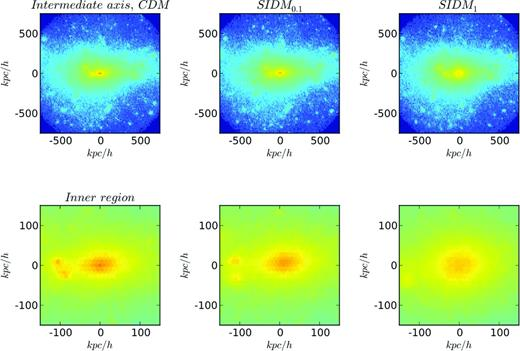
\includegraphics[width=0.8\linewidth]{Figures/dm-models-halo-illus.jpeg}
    \caption{Illustrative differences in the matter distribution within haloes in different models of dark matter. Credit: Annika et al. (2013) \citep{2013MNRAS.430..105P}.}
    \label{fig:dm-models-haloes}
\end{figure}

\section{Cosmological simulations}

These simulations often rely on N-body techniques to solve the non-linear gravitational interactions of a large number of particles in cosmological volumes. They usually take initial conditions produced by perturbative approximations in the linear regime starting from a density fluctuation generated with a given power spectrum. Cosmological simulations, particularly those employing the $\Lambda$CDM model, have been instrumental in studying dark matter haloes. Figure \ref{fig:dm-cosmo-sims-haloes} depicts the matter distribution simulated over a large cosmological volume consisting of a large number of haloes. Such cosmological simulations have revealed several key properties of dark matter haloes. For instance, haloes are generally triaxial in shape \citep[][]{1988ApJ...327..507F} and exhibit a universal density profile described by, for example, the Navarro-Frenk-White (NFW) profile \citep{1996ApJ...462..563N,1997ApJ...490..493N,2010MNRAS.402...21N}.

\begin{figure}
\centering
\includegraphics[width=0.8\linewidth]{Figures/20210910-cfca-fig1-full.jpg}
\caption{The projected dark matter density field, illustrating the distribution of haloes in a cosmological simulation. Credit: Tomoaki Ishiyama.}
\label{fig:dm-cosmo-sims-haloes}
\end{figure}

These simulations also reveal the distribution of these haloes in the cosmic web, such as the halo mass functions and assembly bias and its connection to the matter power spectrum. In addition, they are also useful in understanding the connections between these halo properties with the large-scale environment in which they reside \cite[see e.g.][]{2021MNRAS.503.2053R,2022MNRAS.516.5849R}.

\section{The Role of Dark Matter Haloes in Galaxy Formation}

Dark matter haloes are not only fundamental to cosmology but also to the formation and evolution of galaxies. Within these haloes, gas can cool and condense to form stars and other astrophysical objects \citep{1988MNRAS.234..459S,1998MNRAS.295..319M}. This process of baryonic matter within dark matter haloes is complex and involves various non-gravitational processes such as radiative cooling, star formation, and feedback mechanisms from supernovae and active galactic nuclei (AGN).

Due to the complexity and wide dynamic range of these baryonic processes, it is challenging to study galaxy formation directly from first principles. Instead, semi-analytic models are often used, which incorporate simplified recipes for baryonic processes and are calibrated against observations \citep{2015ARA&A..53...51S}. These models allow for the efficient exploration of different galaxy formation scenarios but they are not as accurate as simulations galaxies that co-evolve with dark matter haloes.

\section{Hydrodynamical Simulations}

The state-of-the-art approach to studying galaxy formation involves numerical hydrodynamical simulations that model both dark matter and baryonic physics within cosmological volumes. Usually, these hydrodynamical simulations, use subgrid models to incorporate processes that occur on scales smaller than the resolution of the simulation. For example, OWLS \citep{2010MNRAS.402.1536S}, Illustris \citep{2014MNRAS.445..175G}, FIRE \citep{2014MNRAS.445..581H}, EAGLE \citep{2015MNRAS.446..521S}, Horizon-AGN \citep[][]{2017MNRAS.467.4739K}, SIMBA \citep[][]{2019MNRAS.486.2827D}, IllustrisTNG \citep{2019ComAC...6....2N} are some of the modern hydrodynamical cosmological (zoom) simulations.

By incorporating radiative cooling, these simulations allow the gas to condense into the center, and when the gas becomes dense enough, some of its mass is converted into stellar particles that collectively track the evolution of a population of stars. This is also associated with the production of gas outflows due to stellar winds and supernovae feedback, enriching the interstellar gas with metals. In addition, they seed central supermassive black holes, forming active galactic nuclei that convert a part of the accreted energy into strong feedback outflows. The formation of such a galaxy in the cosmological setting is depicted in \figref{fig:illustrate-sim-eagle}.

\begin{figure}
\centering
\includegraphics[width=0.7\linewidth]{Figures/eagle_zoom_stages1.png}
\caption{Illustration of the hydrodynamical simulation EAGLE with subgrid baryonic prescriptions producing realistic galaxies in a cosmological volume. Credit: Virgo Consortium.}
\label{fig:illustrate-sim-eagle}
\end{figure}

These subgrid prescriptions often include parameters that are only constrained by comparing against observational data. However, this approach is still one of the most realistic frameworks for studying the coupled evolution of dark matter and baryons in a cosmological setting. In particular, they account for the backreaction of galaxy formation on dark matter haloes, which can significantly alter the haloes' properties. For instance, the shape of dark matter haloes can be affected by the presence of a central galaxy \citep{2010MNRAS.407..435A,2021MNRAS.501.5679C}, which is important for interpreting weak lensing measurements \citep{2021A&A...647A.185G}. Additionally, the concentration and density profiles of dark matter haloes are modified by baryonic processes, influencing the rotation curves of galaxies.


\section{Relaxation response of dark matter haloes}

Any form of dark matter that interacts gravitationally with baryonic matter must have been influenced by the formation and evolution of baryonic galaxies. Hence, the properties of dark matter haloes are determined by both cosmology and the astrophysics of galaxies. Usually, for convenience, the role of cosmology and the exact particle nature of the dark matter on halo properties is investigated separately from the astrophysical effects. The change in the dark matter halo properties due to the inclusion of astrophysical effects is known as the halo response to galaxies. This response of the dark matter haloes has two major aspects: one is the change in the radial distribution, and the other is the angular distribution. While the change in the angular distribution has implications for the shapes of the haloes, the change in the radial distribution affects the spherically averaged mass profiles, which have implications for the rotation curves \citep[][]{2004ApJ...616...16G,2006PhRvD..74l3522G,2010MNRAS.402..776P,2010MNRAS.406..922T,2010MNRAS.405.2161D,2010MNRAS.407..435A,2011MNRAS.414..195T,2016MNRAS.461.2658D,2019A&A...622A.197A,2022MNRAS.511.3910F,2023Velmani&Paranjape}.

In this thesis, we primarily focus on the response in the radial distribution. Early work treated this response using adiabatic invariants \citep[][]{osti6457593,1984MNRAS.211..753B,1986ApJ...301...27B,1987ApJ...318...15R}. Using simplifying assumptions such as spherical symmetry, no shell crossing, and angular momentum conservation with circular orbits for dark matter particles, Blumenthal et al. (1986) \citep[][]{1986ApJ...301...27B} derived a simple formula that quantifies the adiabatic relaxation of the dark matter mass profile in terms of the final baryonic distribution (we discuss this in detail later).

Currently, the most robust technique to understand the consequences of gas assembly and galaxy formation on dark matter structure is the use of high-resolution cosmological hydrodynamical (zoom) simulations, which employ `sub-grid' recipes for galaxy formation. In such simulations, the response of the dark matter to the presence of baryons in a halo can be ascertained by comparing a halo in the full hydrodynamical simulation to a matched `partner' halo in a collisionless, gravity-only simulation performed using the same initial random fluctuations. Using this technique, it was found that a simple adiabatic contraction model \citep[][]{1986ApJ...301...27B} is an inaccurate description of the response in a variety of simulations \citep[see, e.g.,][]{2004ApJ...616...16G,2006PhRvD..74l3522G,2010MNRAS.402..776P,2010MNRAS.406..922T,2010MNRAS.405.2161D,2010MNRAS.407..435A,2011MNRAS.414..195T,2016MNRAS.461.2658D,2019A&A...622A.197A,2022MNRAS.511.3910F}.

Even in a simpler setting, where star formation and feedback effects are ignored, Abadi et al. (2010) \citep{2010MNRAS.407..435A} has shown that the relaxation response of the halo is significantly less than the prediction of the idealized adiabatic relaxation model; this is illustrated in \figref{fig:illustrate_abadi}. For a dark matter shell that changes its radius from $r_i$ to $r_f$, it will be accompanied by a change in the enclosed total mass from $M_i$ to $M_f$. As the condensation of baryons to the center causes $M_i/M_f < 1$, the change in the radius of the dark matter shell, characterized by $r_f/r_i < 1$, is far from the predictions of the idealized model of adiabatic relaxation.

\begin{figure}
\centering
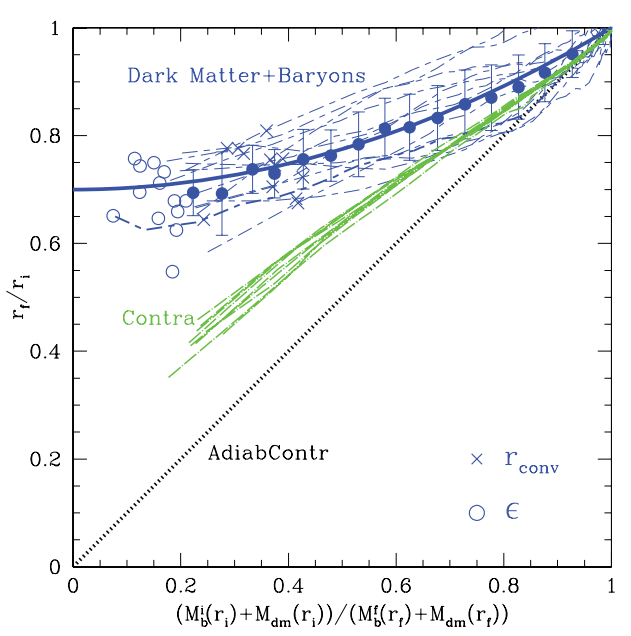
\includegraphics[width=0.7\linewidth]{Figures/Abadi_relxation.png}
\caption{Relaxation response of dark matter haloes to galaxy formation presented by Abadi et al. (2010). The `AdiabContra' line indicates the predictions of an idealized model of adiabatic contraction \citep[][]{1986ApJ...301...27B} and the `Contra' line indicates the prediction of a modified model proposed by Gnedin et al. (2004) \citep{2004ApJ...616...16G}.}
\label{fig:illustrate_abadi}
\end{figure}

Several authors have investigated whether discarding some of the assumptions of the idealized model \citep[][]{1986ApJ...301...27B} can help reconcile with the simulation results. Gnedin et al. (2004) \citep{2004ApJ...616...16G} considered non-spherical orbits for the dark matter particles and suggested a simple modification to the original model. This modified empirical formula shows wide variation in its parameters across haloes from different simulations and at different redshifts \citep[][]{2006PhRvD..74l3522G,2010MNRAS.405.2161D}.

As an alternative approach, Sellwood et al. (2005) \citep[][]{2005ApJ...634...70S} accounted for the random motions within the halo using invariant action integrals, developing on the early works of Young (1980) \citep{1980ApJ...242.1232Y}. This model gives a better approximation of the response even in modern hydrodynamical simulations \citep{2020MNRAS.495...12C}; however, making predictions using this model requires access to orbital phase space information of the halo, which may not always be feasible.

Physically, one expects that the overall response of the halo is mediated by a combination of different astrophysical processes that occur in the galaxy. Feedback processes are known to reduce the contraction of the halo significantly; e.g., supernova-driven winds can completely transform the inner density profile of the dark matter halo \citep[][]{1996MNRAS.283L..72N}. This may be the key in reconciling the observation of dark matter cores at the center of various galaxies with the cuspy haloes found in gravity-only $\Lambda$CDM simulations \citep[see][for a review]{2014Natur.506..171P}. However, such feedback effects do not always produce dark matter cores from cusps. Rather, this can depend on the amount of gas ejected, the mass loss timescale, and the frequency of starburst events (see, e.g., \citealp{2011ApJ...736L...2O,2014ApJ...793...46O,2012MNRAS.421.3464P}, and also \citealp{bfln18}). In massive haloes hosting galaxy groups or clusters, while the formation of powerful AGN in the central galaxy can strongly suppress star formation, it can still significantly reduce the adiabatic contraction of the halo \citep[][]{2011MNRAS.414..195T}. Moreover, the fluctuation in gravitational potential due to such feedback can expel the dark matter from the inner halo, producing inner cores \citep[][]{2012MNRAS.422.3081M}.

% Different aspects of the halo response, such as the change in its mass profile, shape, phase space distribution and substructure population, have been explored to date in a variety of hydrodynamical simulations \citep[see, e.g.,][]{2004ApJ...611L..73K,2008ApJ...681.1076D,2014MNRAS.441.2986D,2015MNRAS.451.1247S,2017MNRAS.466.3876Z,2017MNRAS.472.4343C,2019MNRAS.484..476C,2021arXiv210900012C,2021MNRAS.501.5679C,2020MNRAS.494.4291C,freundlich+20,riggs+22}.
% A detailed understanding of the formation and evolution of galaxies and their interaction with their environment is a pressing open problem. 

% The goal of this chapter is to perform a systematic, statistical study of this dark matter response in high-resolution hydrodynamical simulations incorporating realistic feedback and quantify it using simple analytical forms, including the sensitivity of this response to halo-centric distance and halo and galaxy properties. To this end, we use the publicly available suites of simulations from the IllustrisTNG and EAGLE projects. 


\section{Self-similar evolution}

An alternate approach to studying the formation and evolution of haloes and galaxies is through the use of self-similar models. While this is not as accurate in producing realistic haloes or galaxies like the full hydrodynamical simulations, it provides more tractable analytical models that offer insights into key features. The key assumption is that the model is `self-similar', so that spatial variations are related to temporal variations through a scale radius that evolves over time. This reduces the nonlinear coupled partial differential equations into ordinary differential equations.

\begin{figure}
\centering
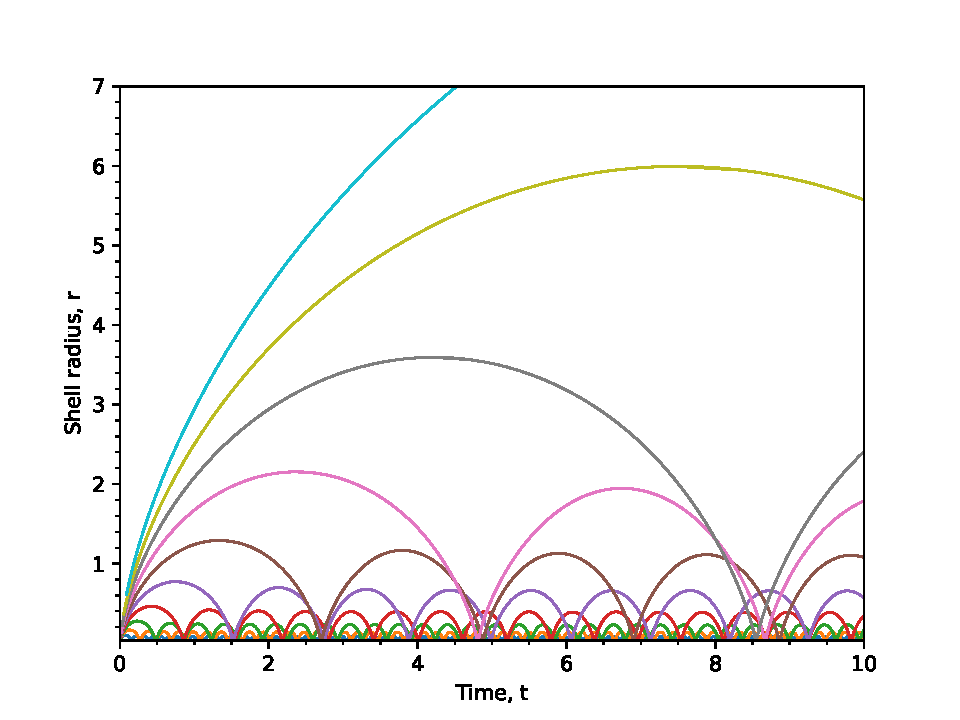
\includegraphics[width=0.8\linewidth]{Figures/illustrate_self-sim_DM_shells.pdf}
\caption{Illustration of the self-similar accretion of collisionless dark matter shells onto a dark matter halo}
\label{fig:self_sim_illustrate}
\end{figure}

In such self-similar systems, the trajectory of different shells of matter are related to each other by a corresponding normalisation factor. This is illustrated in \figref{fig:self_sim_illustrate} for the self-similar accretion onto a dark matter halo. At any given point in time, some of the shells are infalling towards the centre while some others are expanding outwards. However, since the dark matter here is collisionless, the shells freely cross through each other. The radial distribution of the dark matter at any given time, is then simply the sum of masses carried by all those shells. This implies, that the radial mass profile at a given time across the range of halo-centric distances describes the mass profile at any other time by normalisation factor.

The self-similar model was pioneered by Fillmore and Goldreich (1984) \cite{1984FillmoreGoldreich} and Bertschinger (1985) \cite{1985Bertschinger}. While Bertschinger devised spherical self-similar solutions for the collapse of dark matter and shocked gas within the Einstein-de Sitter (EdS) universe, under the assumption of a constant accretion rate, Fillmore and Goldreich explored self-similar solutions for the collapse of dark matter from various initial mass distributions, expanding their purview to include not only spherical but also cylindrical and planar self-similar collapses. 

Extending those works, Bertschinger (1989) \citep{1989Bertschinger} also studied self-similar cooling flows of gas, focusing on the inner regions of galaxies. In contrast, Owen et al. (1998) \citep{1998OwenWeinberg_etal} derived a set of cooling functions that guarantee self-similar evolution by ensuring that the cooling time-scale remains a constant fraction of the Hubble time in an object with a characteristic clustering mass. Abadi et al. (2000) \citep{2000Abadi_etal_SelfSimCool} studied the self-similar accretion of gas with radiative cooling in the EdS Universe.

Later on, Shi (2016a) \cite{2016ShiDMLamCDM} generalised self-similar models to $\Lambda$CDM models, focusing on the outer profile and, notably, the outermost caustic or `splashback radius' of dark matter collapse which has gained recent popularity \cite{2014DiemerKrastov,2014AdhikariDalalChamberlain,2018Changetal_DES_splashback}.
In a complementary study, Shi (2016b) \cite{2016ShiICM} probed the self-similar accretion of shocked gas, dissecting its behavior with respect to accretion rates and revealing correlations between the shock radius of gas and the dark matter's splashback radius. In general, the self-similar assumption offers a powerful tool to simplify the problem and render it more tractable.



% \section{Open Problems and Research Motivation}
\section{Objectives}

In this thesis, we perform a comprehensive investigation of the interplay between galaxy formation and its host halo evolution, focusing on the changes in the radial distribution of dark matter in response to galaxy formation and evolution. Through state-of-the-art galaxy formation simulations, we investigate the exact nature of the relaxation response and its dynamical evolution along with its connection to various galaxy and halo properties. To complement this, we also study the relaxation response by building a more tractable self-similarly evolving systems of individual galaxies with their host haloes. This unified picture of the role of various galactic astrophysical processes in mediating the response of dark matter haloes also provides useful timescales for predicting dynamical changes in radial mass profiles caused by astrophysical effects.

Understanding the nature of this response (or `baryonic backreaction') is critical in building accurate and robust models of dark matter haloes, for use in interpreting the results of upcoming large-volume surveys (\citealp{2015JCAP...12..049S,2018MNRAS.480.3962C,2021MNRAS.503.3596A}; see also \citealp{velliscig+14,hwvh15,mead+15}) as well as the detailed prediction of rotation curves and related statistics \citep{2021MNRAS.507..632P,2022MNRAS.517..130P}. In addition, understanding the dynamical behaviour of the dark haloes during the evolution of the galaxies they host is a key ingredient needed for building a complete picture of galaxy evolution.

From the cosmological perspective, the effects of baryons are often considered nuisances in the inference of fundamental cosmological parameters. For instance, feedback from AGN can mimic the effects of other cosmological parameters, such as the presence of massive neutrinos or warm dark matter candidates, at certain scales \citep{2019Chisari_etal_Baryfeedback,2020AricoAnguloetal_baryonifi}. Distinguishing between these effects requires a detailed understanding of baryonic processes and their impact on dark matter.



% In the standard paradigm of the $\Lambda$CDM cosmology, dark matter haloes are formed from the gravitational collapse around initial overdensities - Galaxies are then formed the baryonic matter within the haloes - dark halo response to the galaxy formation - literature on adiabatic relaxation.

% \section{Current status}



% \subsection{Dark matter haloes}

% \subsection{Cosmological simulations}

% \subsection{Simulations with galaxy formation}

% \subsection{Relaxation response of dark matter}

% \section{Objective}

% \section{Quasi-adiabatic relaxation}

% \section{Self-similar systems}
% \cite{2015LauNagaietal}

% \section{Motivation}

% \section{Dynamical relaxation}

% \section{Outline}

\section*{Organization of the Thesis}

\begin{itemize}
    \item In the first chapter of this thesis, we review the background material and define the primary objectives, along with their relevance to the broader context.
    
    \item In the second chapter, we demonstrate the specific techniques we employed in studying the simulated response of dark matter haloes to galaxy formation and evolution within simulations of cosmological volumes.
    
    \item In the third chapter, we present our findings from state-of-the-art galaxy formation simulations, IllustrisTNG and EAGLE, characterizing the dark matter response in a wide variety of haloes at present epoch. We introduce novel fitting functions that accurately describe this relaxation response, revealing an additional dependence on halo-centric distance and highlighting the significant role of star formation-related feedback processes.
    
    \item In the fourth chapter, we explore the role of astrophysical modeling in producing the halo response at different epochs in simulations. We find the gas equation of state to have significant influence in EAGLE haloes, and we also quantify the strong influence of AGN and stellar feedback in CAMELS simulations. Our results show a more universal relaxation response at an earlier epoch ($z=1$) compared to $z=0$. These findings are applicable to semi-analytical tools for modeling galactic and large-scale structures.
    
    \item In the fifth chapter, we uncover the causal connections between star formation activities, feedback processes, and halo relaxation. Through time-series analyses, we provide new insights into the immediate and delayed effects across different halo regions. Our estimates of the timescales can potentially improve the description of halo profiles in existing baryonification schemes and semi-analytical galaxy formation models.

    \item In the sixth chapter, we develop a spherical self-similar model for galaxy formation that simultaneously and self-consistently solves for the evolution of gas and dark matter, producing pseudo galaxy disks within the halo. This complementary approach offers a framework to rapidly explore the sensitivity of halo response to various astrophysical processes. We find quasi-adiabatic halo relaxation similar to full non-linear simulations, with similarly strong trends related to the gas equation of state.

    \item In the seventh chapter, we summarize the key findings of this thesis and discuss the future outlook.
\end{itemize}